%!TEX root = ../main.tex
% APÉNDICE F — Diagramas UML
% Fuentes PlantUML en figuras/uml/*.puml (estilo común en _estilo.iuml). Para regenerar:
%   java -jar plantuml.jar -tsvg -charset UTF-8 figuras/uml/0*.puml   (requiere Graphviz)
%   rsvg-convert -f pdf -o figuras/uml/X.pdf figuras/uml/X.svg

\chapter{Diagramas UML}\label{apx:uml}

Este apéndice modela \sistema{} con nueve diagramas UML. Complementan la
arquitectura del capítulo~\ref{cap:marco-tecnologico}
(sección~\ref{sec:infraestructura}, tabla~\ref{tab:componentes} y
figura~\ref{fig:arquitectura}) y el modelo de datos de la
sección~\ref{sec:modelo-datos}, sin repetir sus justificaciones: las
diferencias entre el diseño inicial y lo implementado se registran en la
sección~\ref{sec:decisiones-implementacion}. Los nombres de clases,
estados, eventos, trabajos programados y \emph{endpoints} que aparecen son
los del código del sistema --el backend en Spring Boot, el frontend en
Next.js y el motor de \gls{matching} en Python--, publicado en los
repositorios del anexo~\ref{anx:repositorios}. Las fuentes editables, en
PlantUML, están en \path{figuras/uml/}.

Los plazos que muestran los diagramas (15 minutos para pagar, sala en
T$-$5, no-show en T$+$10, corte automático 5 minutos después del fin
agendado, 24 horas de ventana de \gls{escrow}) salen de la Tabla de
Tiempos del sistema. La ventana mínima de anticipación para reservar se
nombra sin cifra, porque es un parámetro de esa tabla que se ajusta con la
operación.

\section{Diagrama de actividad}

La figura~\ref{fig:uml-actividad} recorre el ciclo completo de una clase,
desde la búsqueda hasta la calificación, con tres carriles: quien paga
(Estudiante adulto o Adulto Responsable), el backend de \sistema{} y el
tutor. Si la clase la pide un menor, la crea como Solicitud de Sesión y su
Adulto Responsable la aprueba; el adulto también puede reservar
directamente para su menor. Antes de crear la Reserva se exige que el
tutor tenga su cuenta de MercadoPago conectada por \gls{oauth}, porque el
cobro se hace con su token y el dinero entra a su cuenta (ADR-M5-02); la
Transacción queda en \path{retenido_escrow}, que en este modelo es una
ventana lógica en la que \sistema{} todavía puede reembolsar. El diagrama
distingue el cierre manual (botón Finalizar) del corte automático, que es
el único que aplica el umbral del 50\,\% de duración efectiva para
separar una sesión finalizada de una interrumpida con reembolso total.
El resumen corre solo si se contrató el adicional, que existe únicamente
entre adultos.

\begin{figure}[H]
    \centering
    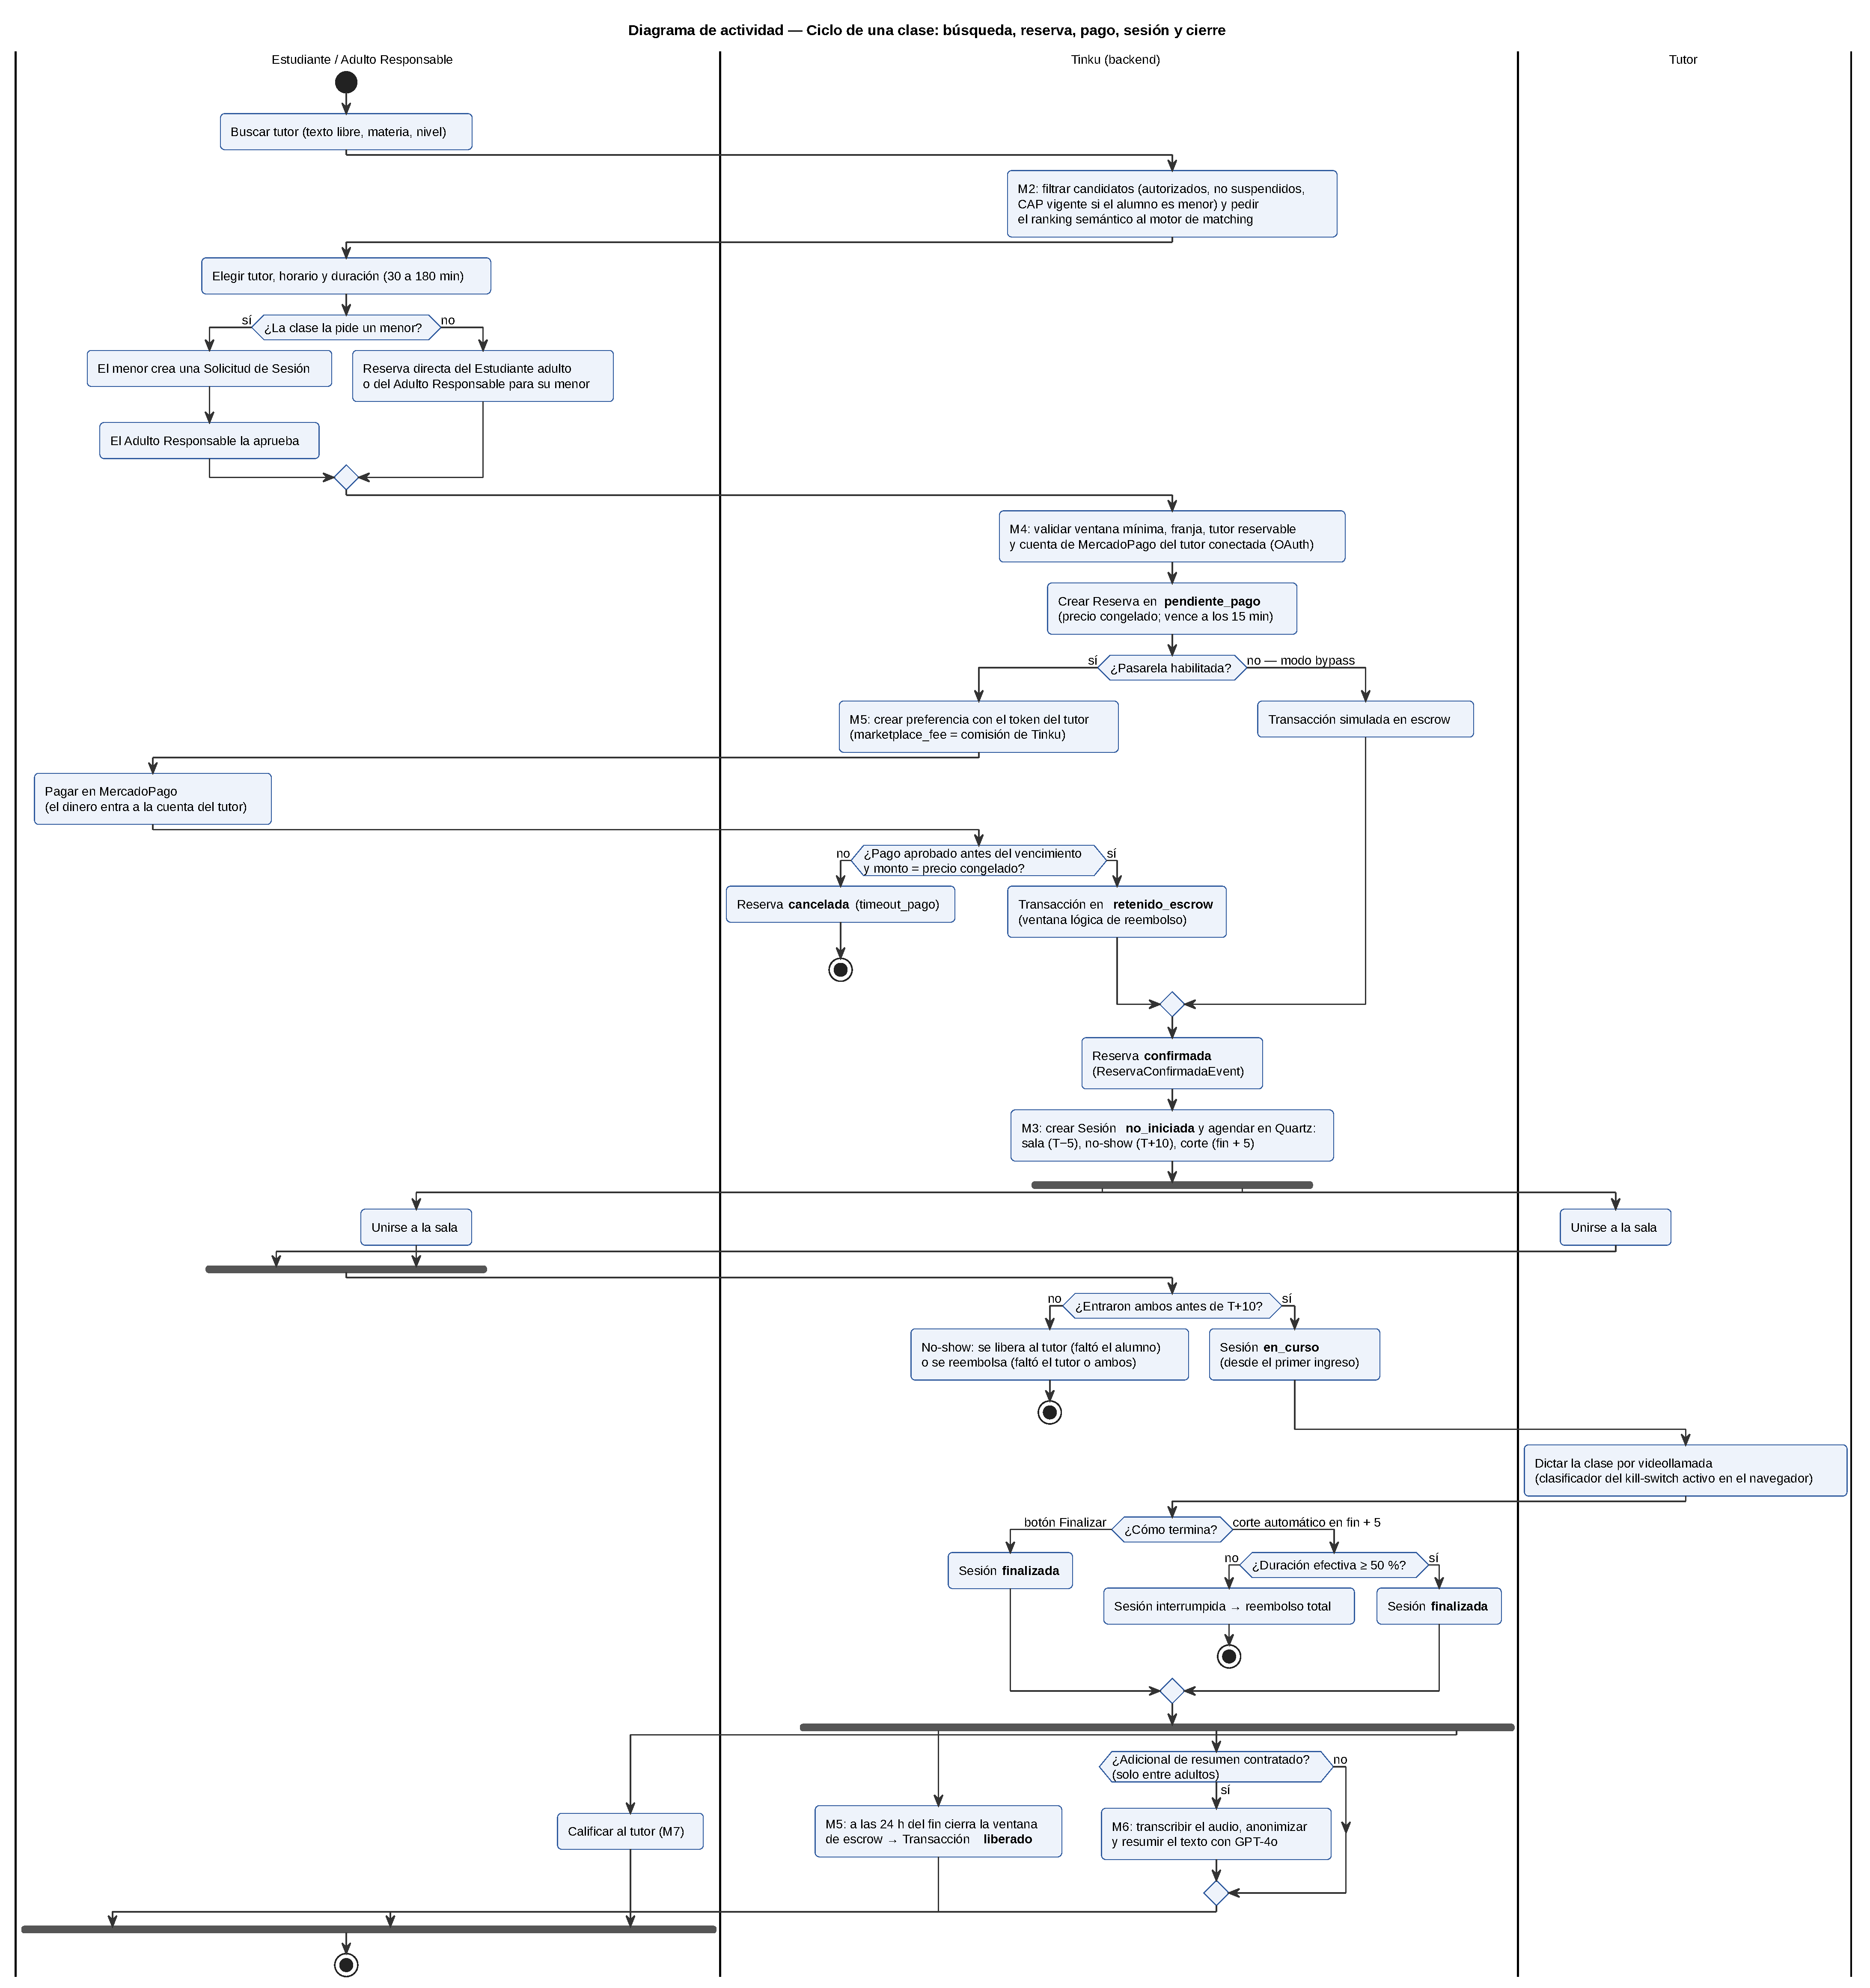
\includegraphics[width=\textwidth,height=0.8\textheight,keepaspectratio]{figuras/uml/01-actividad-reserva}
    \caption{Diagrama de actividad: ciclo de una clase}
    \label{fig:uml-actividad}
\end{figure}

\section{Diagrama de casos de uso}

La figura~\ref{fig:uml-casos-uso} muestra los actores humanos y los
sistemas externos (MercadoPago, LiveKit Cloud y OpenAI). Estudiante
adulto, Adulto Responsable, Estudiante menor y tutor especializan a
Usuario registrado; el Visitante solo puede registrarse, porque la
búsqueda y los perfiles requieren una sesión iniciada. El menor busca,
solicita sesiones y participa en el aula, pero no paga, no autoriza
tutores ni denuncia. Los administradores no son un tipo de usuario: se
modelan como dos actores, uno por rol (Moderación y Seguridad, Soporte
Financiero), como se describe en la sección~\ref{sec:modelo-datos}. El
kill-switch no lo acciona una persona: es una detección automática del
clasificador que corre en el navegador y extiende la participación en el
aula; entre adultos, la contraparte confirma o descarta la detección.

\begin{figure}[H]
    \centering
    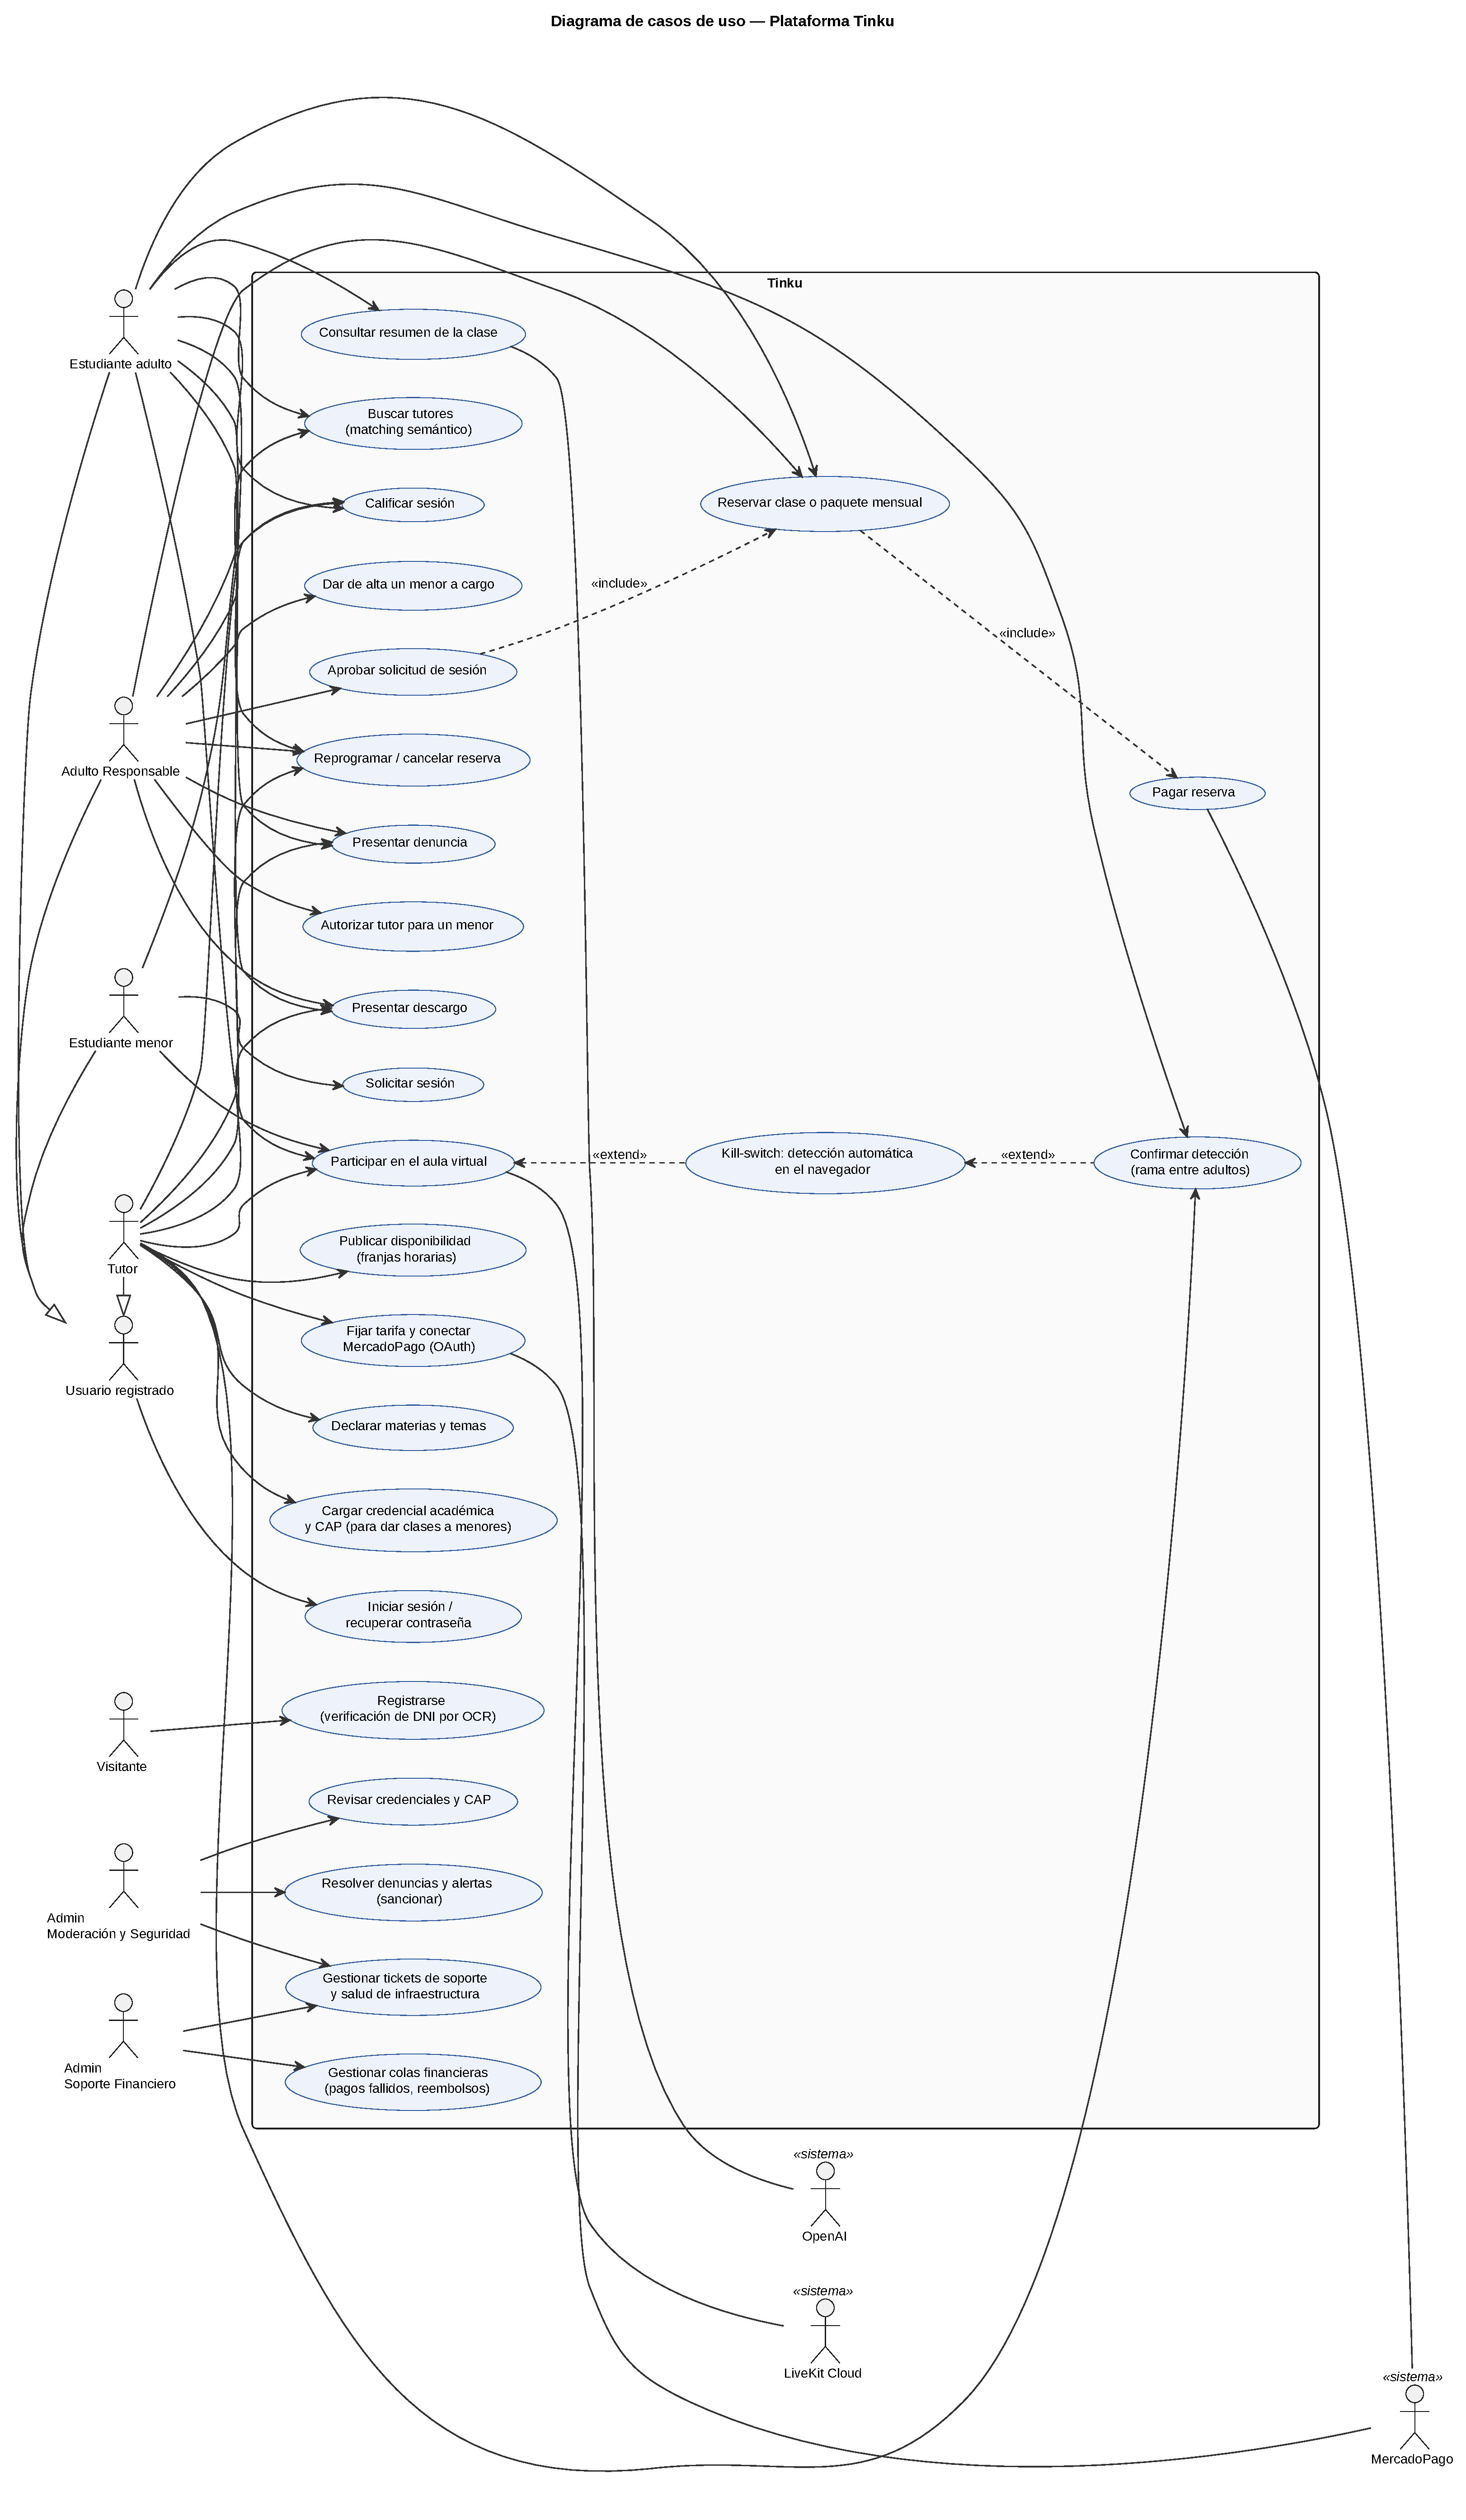
\includegraphics[width=\textwidth,height=0.8\textheight,keepaspectratio]{figuras/uml/02-casos-de-uso}
    \caption{Diagrama de casos de uso de \sistema{}}
    \label{fig:uml-casos-uso}
\end{figure}

\section{Diagramas de máquina de estados}

La figura~\ref{fig:uml-estados-reserva} modela \texttt{EstadoReserva}. Una
Reserva nace en \path{pendiente_pago} y pasa a \texttt{confirmada} cuando
el pago se aprueba por cualquiera de sus vías (aviso de MercadoPago,
vuelta del navegador, conciliación periódica o modo \emph{bypass}). El
cambio de horario no la saca de \texttt{confirmada} y nunca la cancela;
la cancelación la decide el pagador, el tutor o el propio sistema (sanción,
baja del menor o \gls{cap} vencido). Termina en \texttt{finalizada},
\texttt{cancelada} o en alguno de los tres estados de no-show. Mientras la
clase transcurre, la Reserva sigue en \texttt{confirmada}: el estado en
vivo lo lleva la Sesión de Aprendizaje, y el valor \path{en_curso} del
enumerado queda reservado.

La figura~\ref{fig:uml-estados-sesion} completa el modelo con los estados
de la Sesión de Aprendizaje y de la Transacción. La sesión pasa a
\path{en_curso} con el primer ingreso; el no-show y el corte automático
con el par roto antes del fin agendado la dejan en
\path{finalizada_anticipada}. En la Transacción, una denuncia pausa el
\gls{escrow} y su resolución lo destraba según el resultado (infundada:
vuelve a contar las 24 horas; fundada: se libera al tutor; escalada: se
reembolsa); el kill-switch lo aparta en \path{pausado_alerta}, que prevalece
sobre la denuncia y termina en reembolso total al resolverse la Alerta.

\begin{figure}[H]
    \centering
    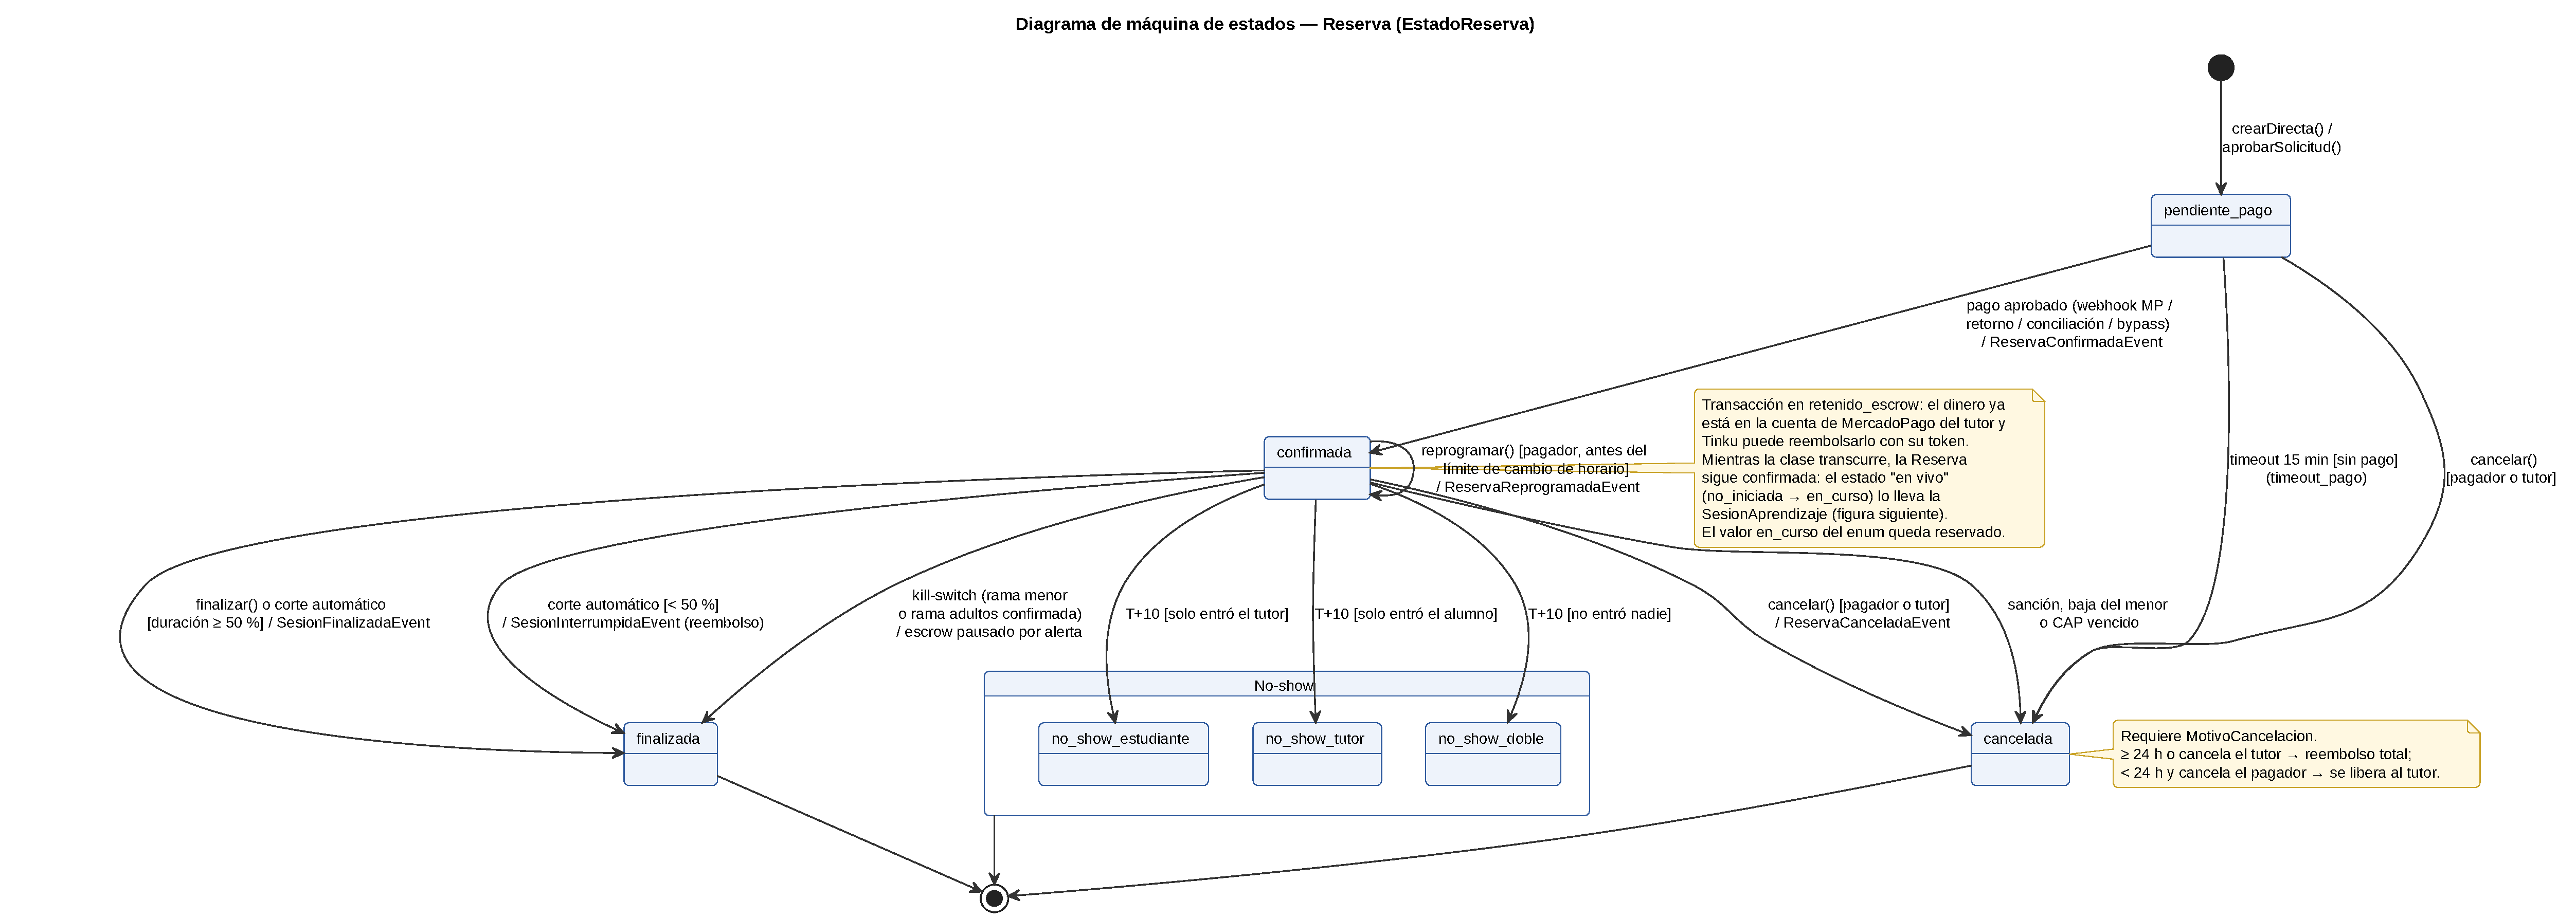
\includegraphics[width=\textwidth,height=0.8\textheight,keepaspectratio]{figuras/uml/03-maquina-estados-reserva}
    \caption{Diagrama de máquina de estados de la Reserva}
    \label{fig:uml-estados-reserva}
\end{figure}

\begin{figure}[H]
    \centering
    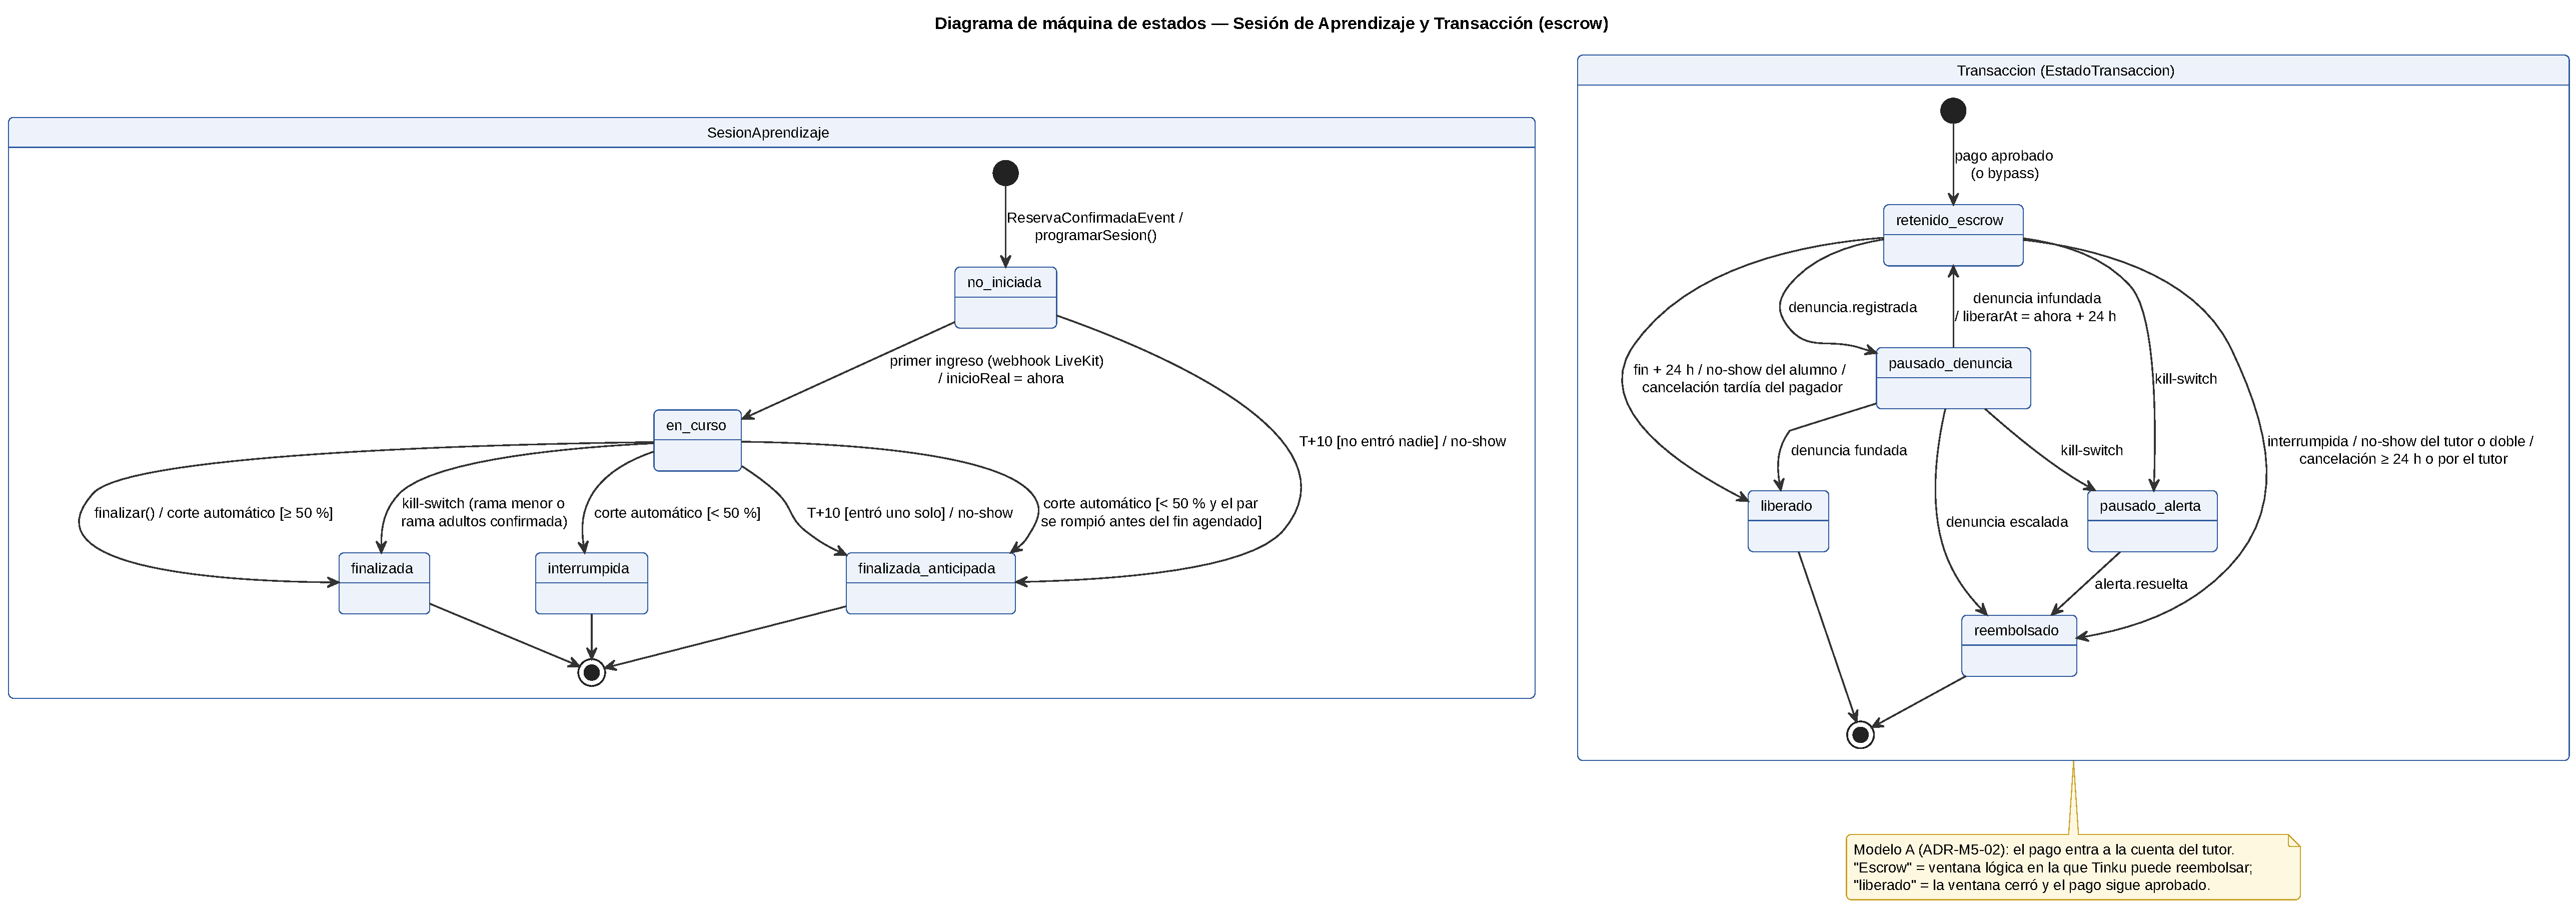
\includegraphics[width=\textwidth,height=0.8\textheight,keepaspectratio]{figuras/uml/03b-maquina-estados-sesion}
    \caption{Diagrama de máquina de estados de la Sesión de Aprendizaje y de la Transacción}
    \label{fig:uml-estados-sesion}
\end{figure}

\section{Diagrama de secuencia}

La figura~\ref{fig:uml-secuencia} detalla la reserva directa y el pago. El
frontend crea la Reserva y pide la preferencia de MercadoPago, que el
backend genera con el token \gls{oauth} del tutor y con la comisión de
\sistema{} como \texttt{marketplace\_fee}. El aviso firmado llega a
\texttt{MercadoPagoWebhookController}, que verifica la firma y resuelve el
token del tutor; \texttt{EscrowService} vuelve a consultar el pago con un
cliente HTTP propio (sin \gls{sdk}), bloquea la fila de la Reserva y, si
el monto coincide con el precio congelado, crea la Transacción en
\path{retenido_escrow} y confirma la Reserva. Con esa confirmación se
publica el evento \texttt{ReservaConfirmadaEvent}, a partir del cual el
módulo de aula crea la Sesión y agenda sus trabajos. Si no llegan ni el aviso ni la vuelta del
navegador, la conciliación periódica sigue el mismo camino.

\begin{figure}[H]
    \centering
    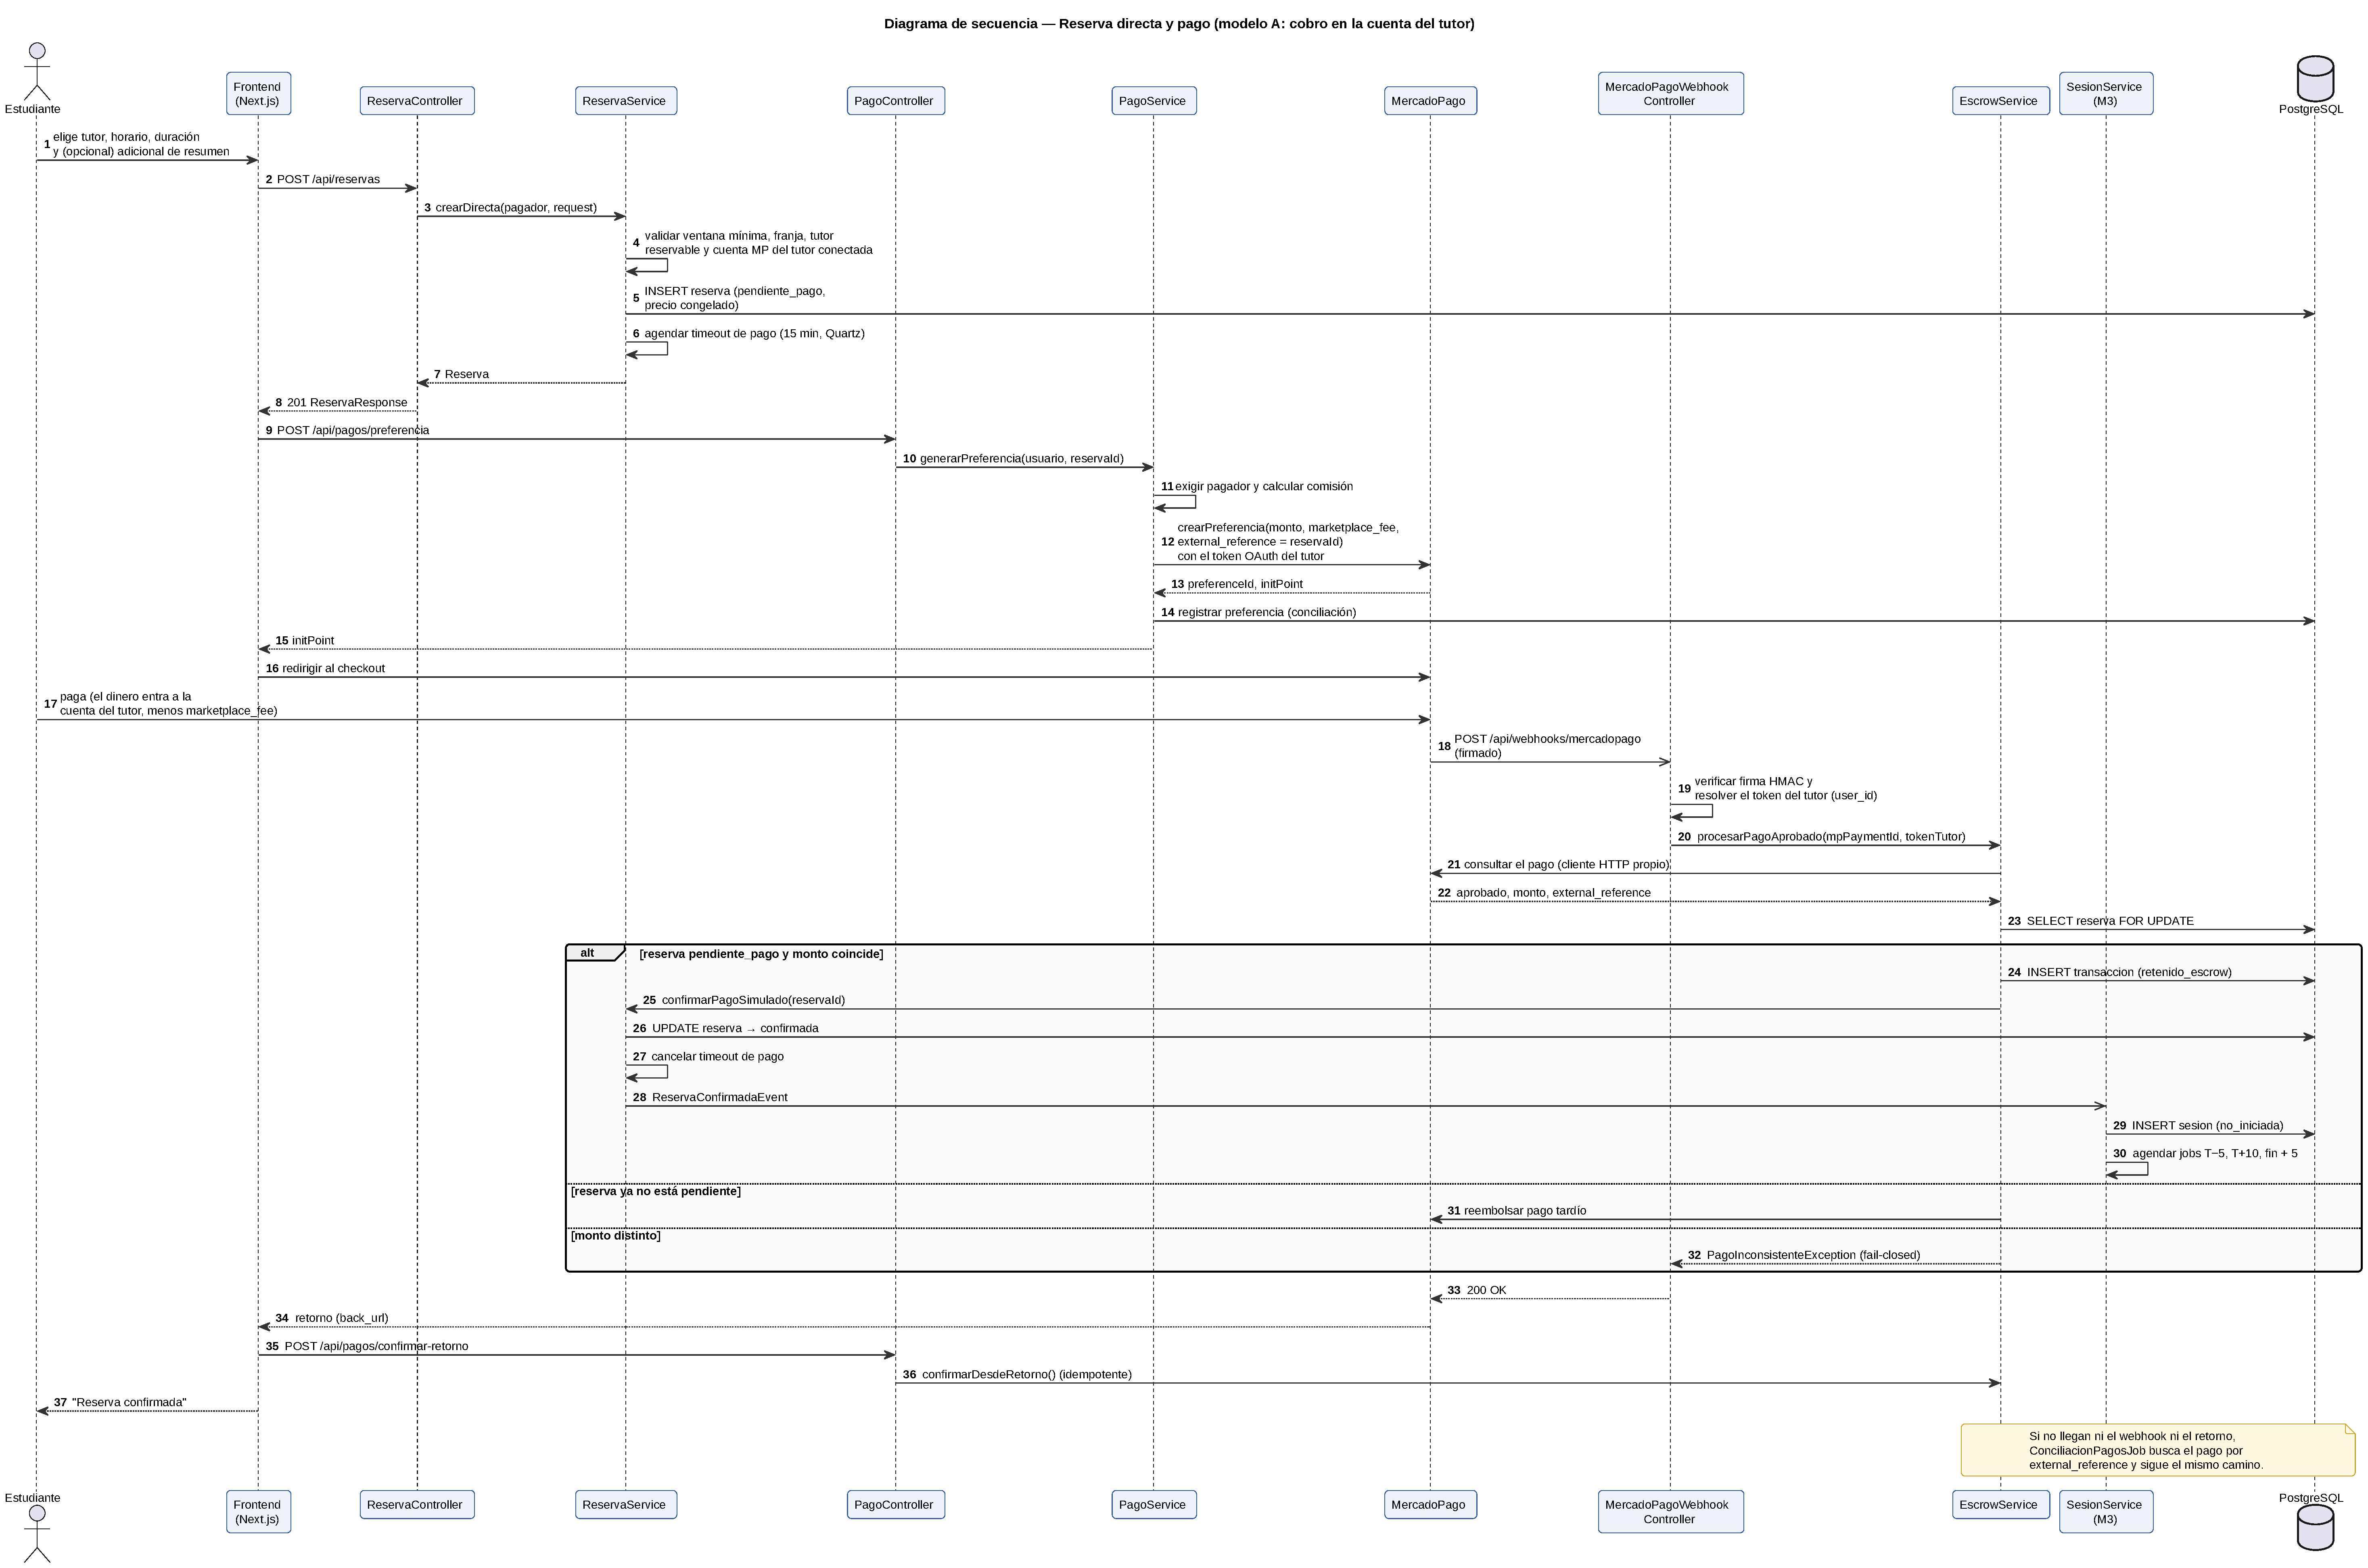
\includegraphics[width=\textwidth,height=0.8\textheight,keepaspectratio]{figuras/uml/04-secuencia-reserva-pago}
    \caption{Diagrama de secuencia: reserva directa y pago}
    \label{fig:uml-secuencia}
\end{figure}

\section{Diagrama de comunicación}

La figura~\ref{fig:uml-comunicacion} muestra, con mensajes numerados, los
objetos que colaboran en el aula virtual: la emisión del token de LiveKit
(que, con un menor, exige que el clasificador del navegador esté listo),
los \emph{webhooks} de ingreso y salida, la cancelación del trabajo de
no-show, el disparo del kill-switch (mensajes K1 a K4, que cierran la
sala) y el corte automático, junto con los eventos que reciben los
módulos de pagos y de resumen.

\begin{figure}[H]
    \centering
    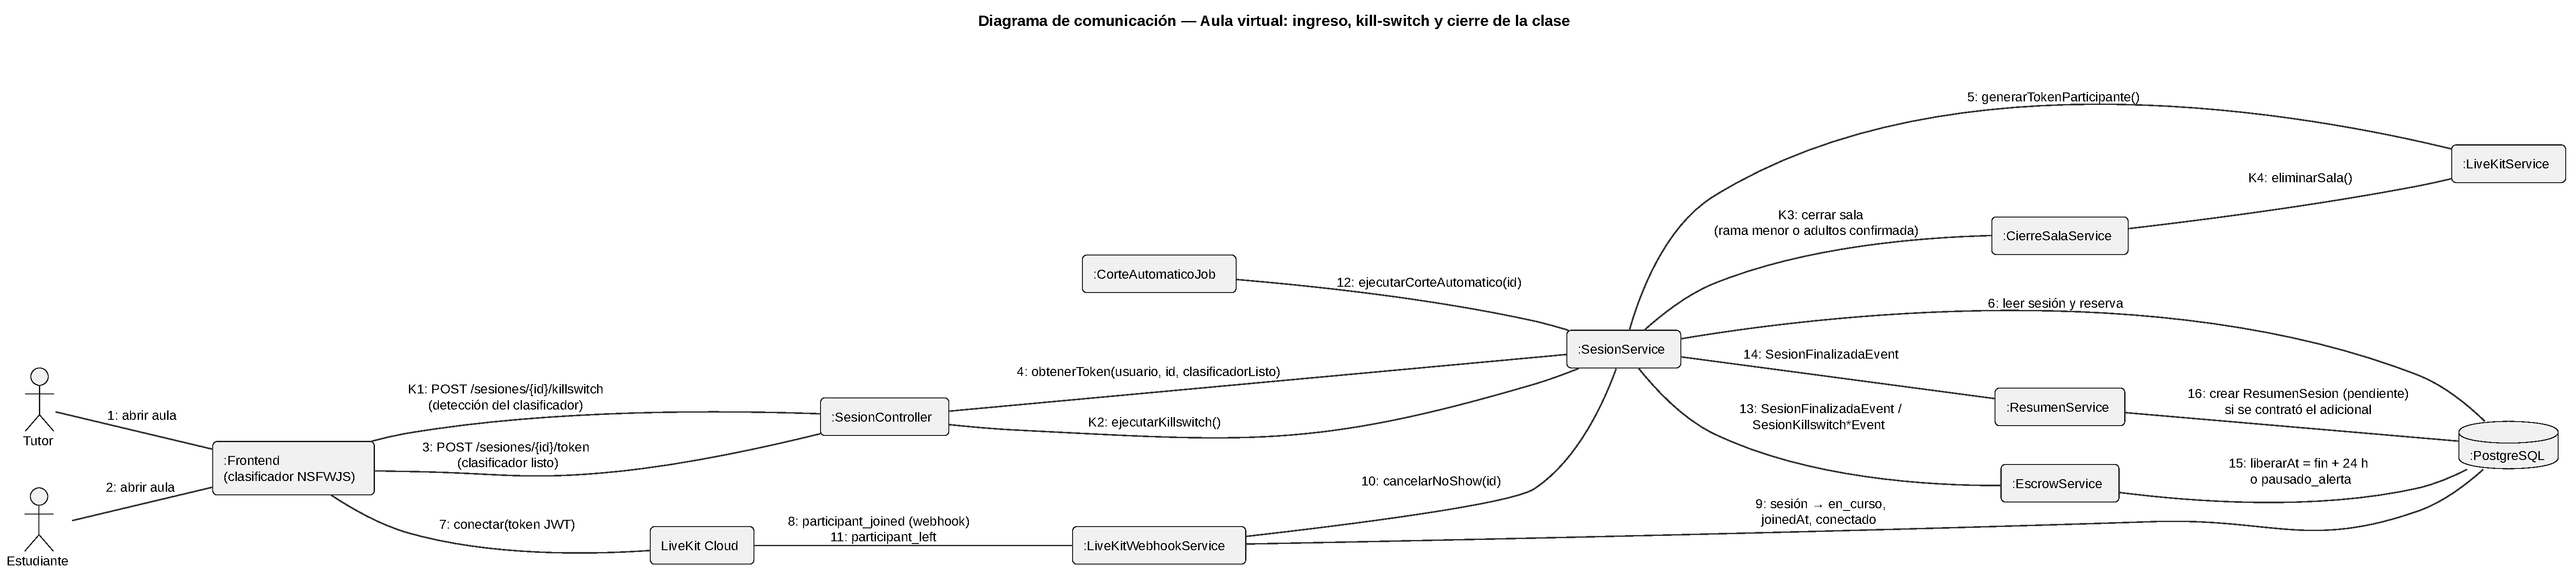
\includegraphics[width=\textwidth,height=0.8\textheight,keepaspectratio]{figuras/uml/05-comunicacion-aula}
    \caption{Diagrama de comunicación: aula virtual}
    \label{fig:uml-comunicacion}
\end{figure}

\section{Diagrama de tiempos}

La figura~\ref{fig:uml-tiempos} ubica en una línea de tiempo los plazos de
una clase de 60 minutos: pago dentro de los 15 minutos, creación de la
sala en T$-$5, decisión de no-show en T$+$10 y corte automático 5 minutos
después del fin agendado. La sesión pasa a \path{en_curso} con el primer
ingreso, y al cierre se fija \texttt{liberarAt} 24 horas después del fin
efectivo de la clase.

\begin{figure}[H]
    \centering
    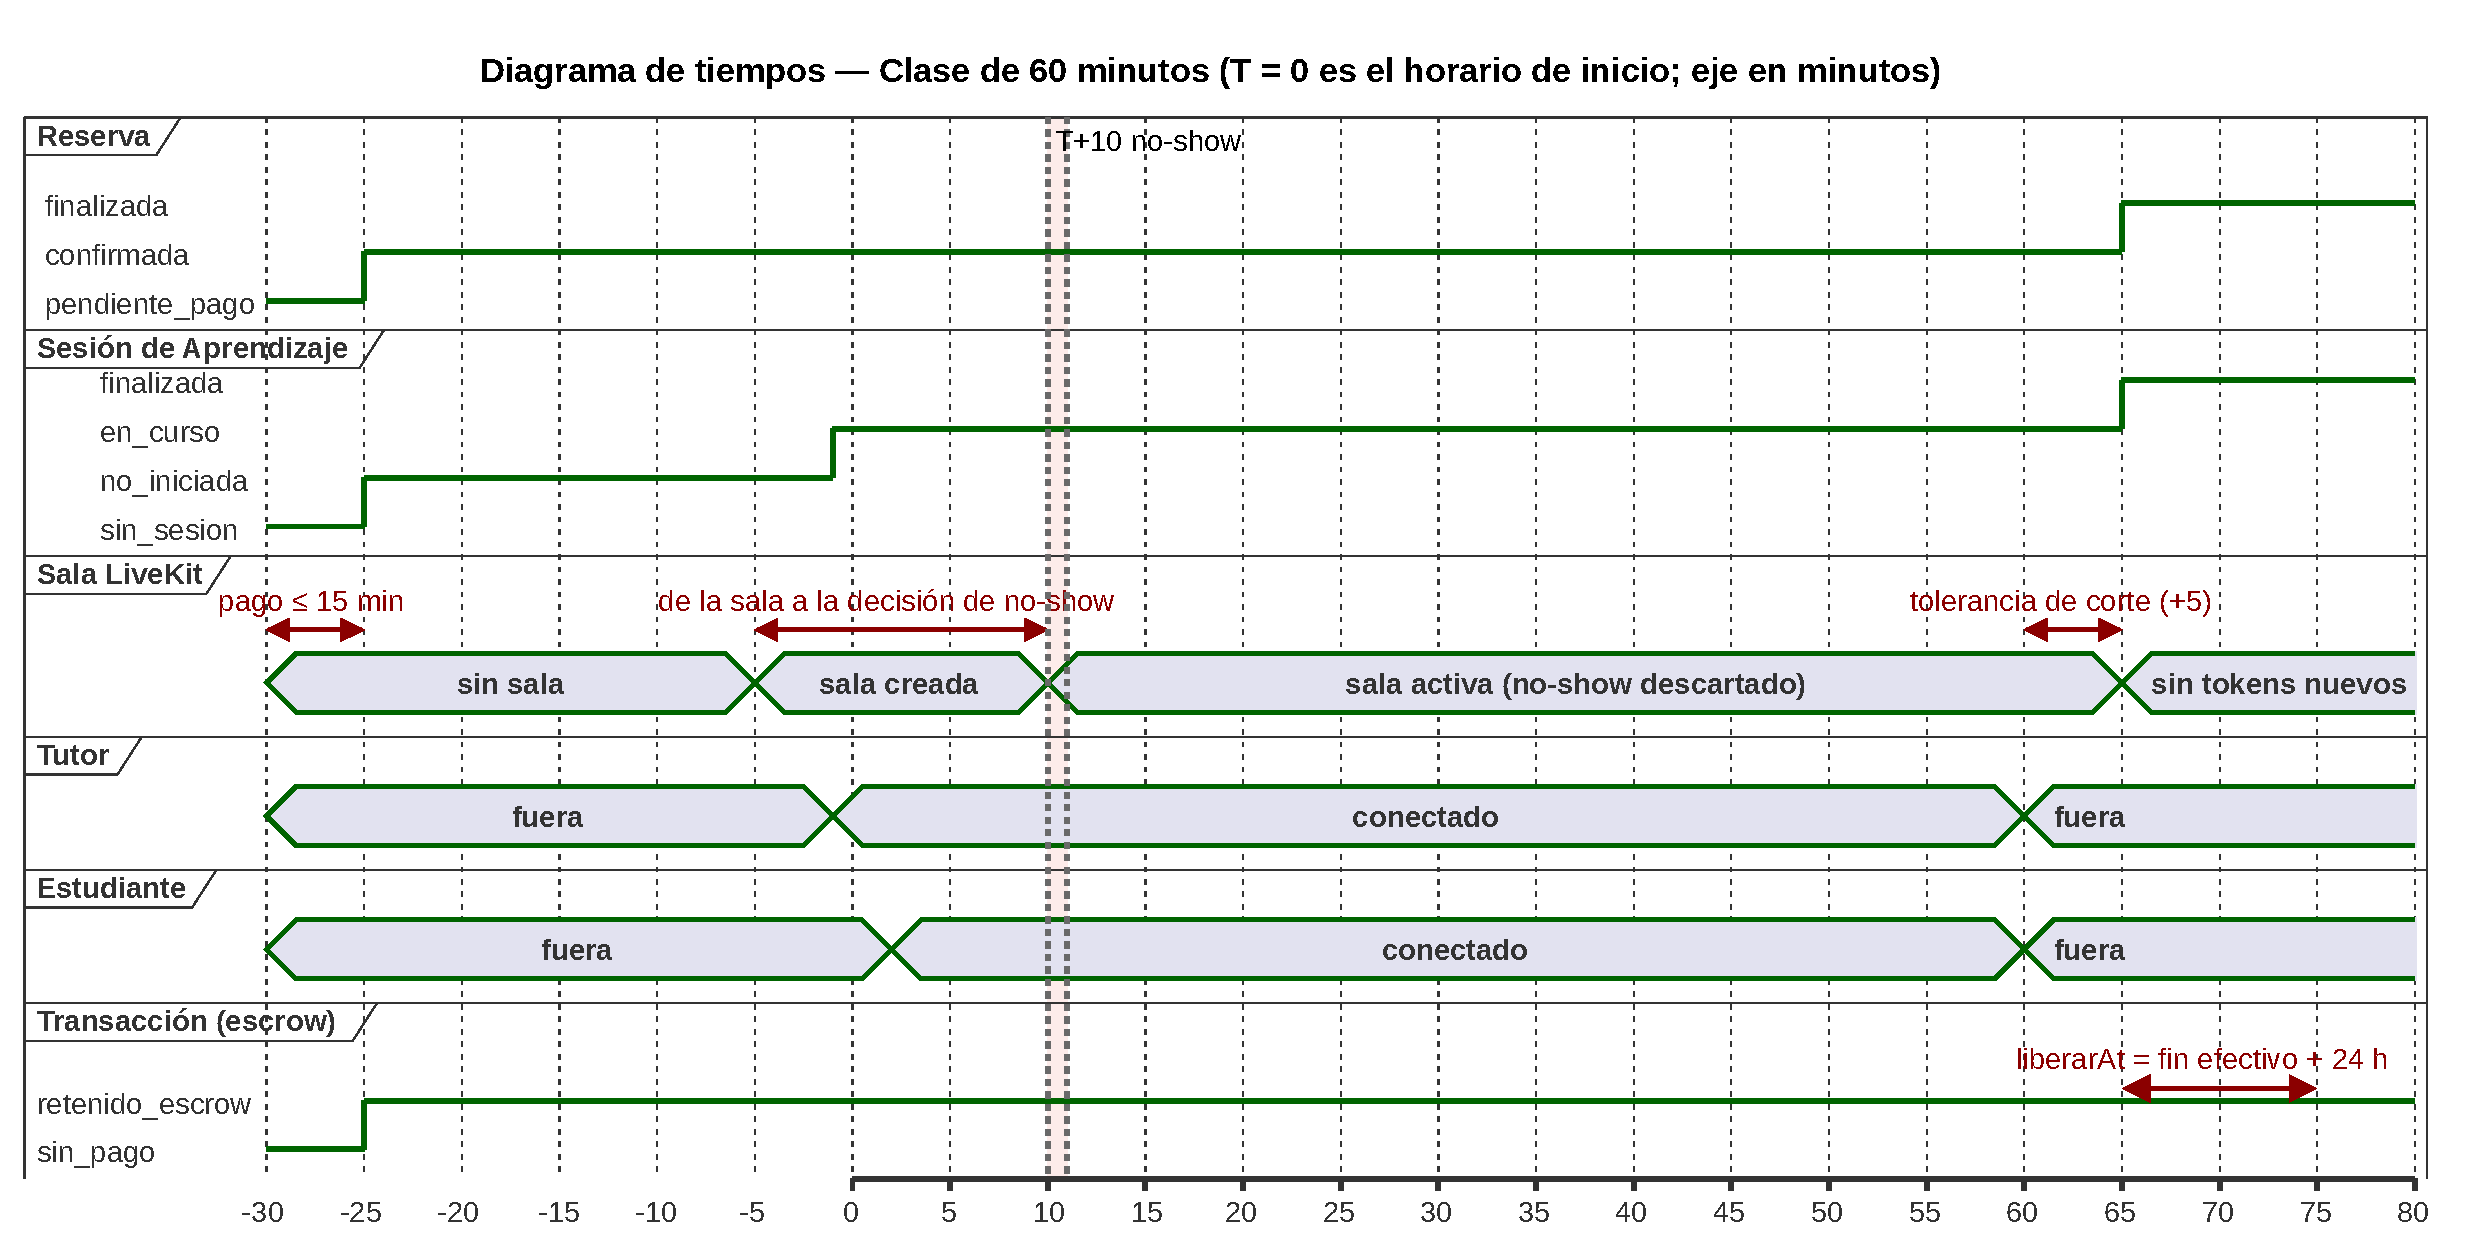
\includegraphics[width=\textwidth,height=0.8\textheight,keepaspectratio]{figuras/uml/06-tiempos-sesion}
    \caption{Diagrama de tiempos de una sesión}
    \label{fig:uml-tiempos}
\end{figure}

\section{Diagrama de visión general de interacciones}

La figura~\ref{fig:uml-vision-general} encadena las interacciones del
sistema como fragmentos \texttt{ref}: búsqueda, solicitud o reserva
directa, pago, ingreso al aula, no-show o kill-switch, cierre y, en
paralelo, el cierre de la ventana de \gls{escrow} (que verifica en
MercadoPago que el pago siga aprobado), el resumen automático y la
calificación.

\begin{figure}[H]
    \centering
    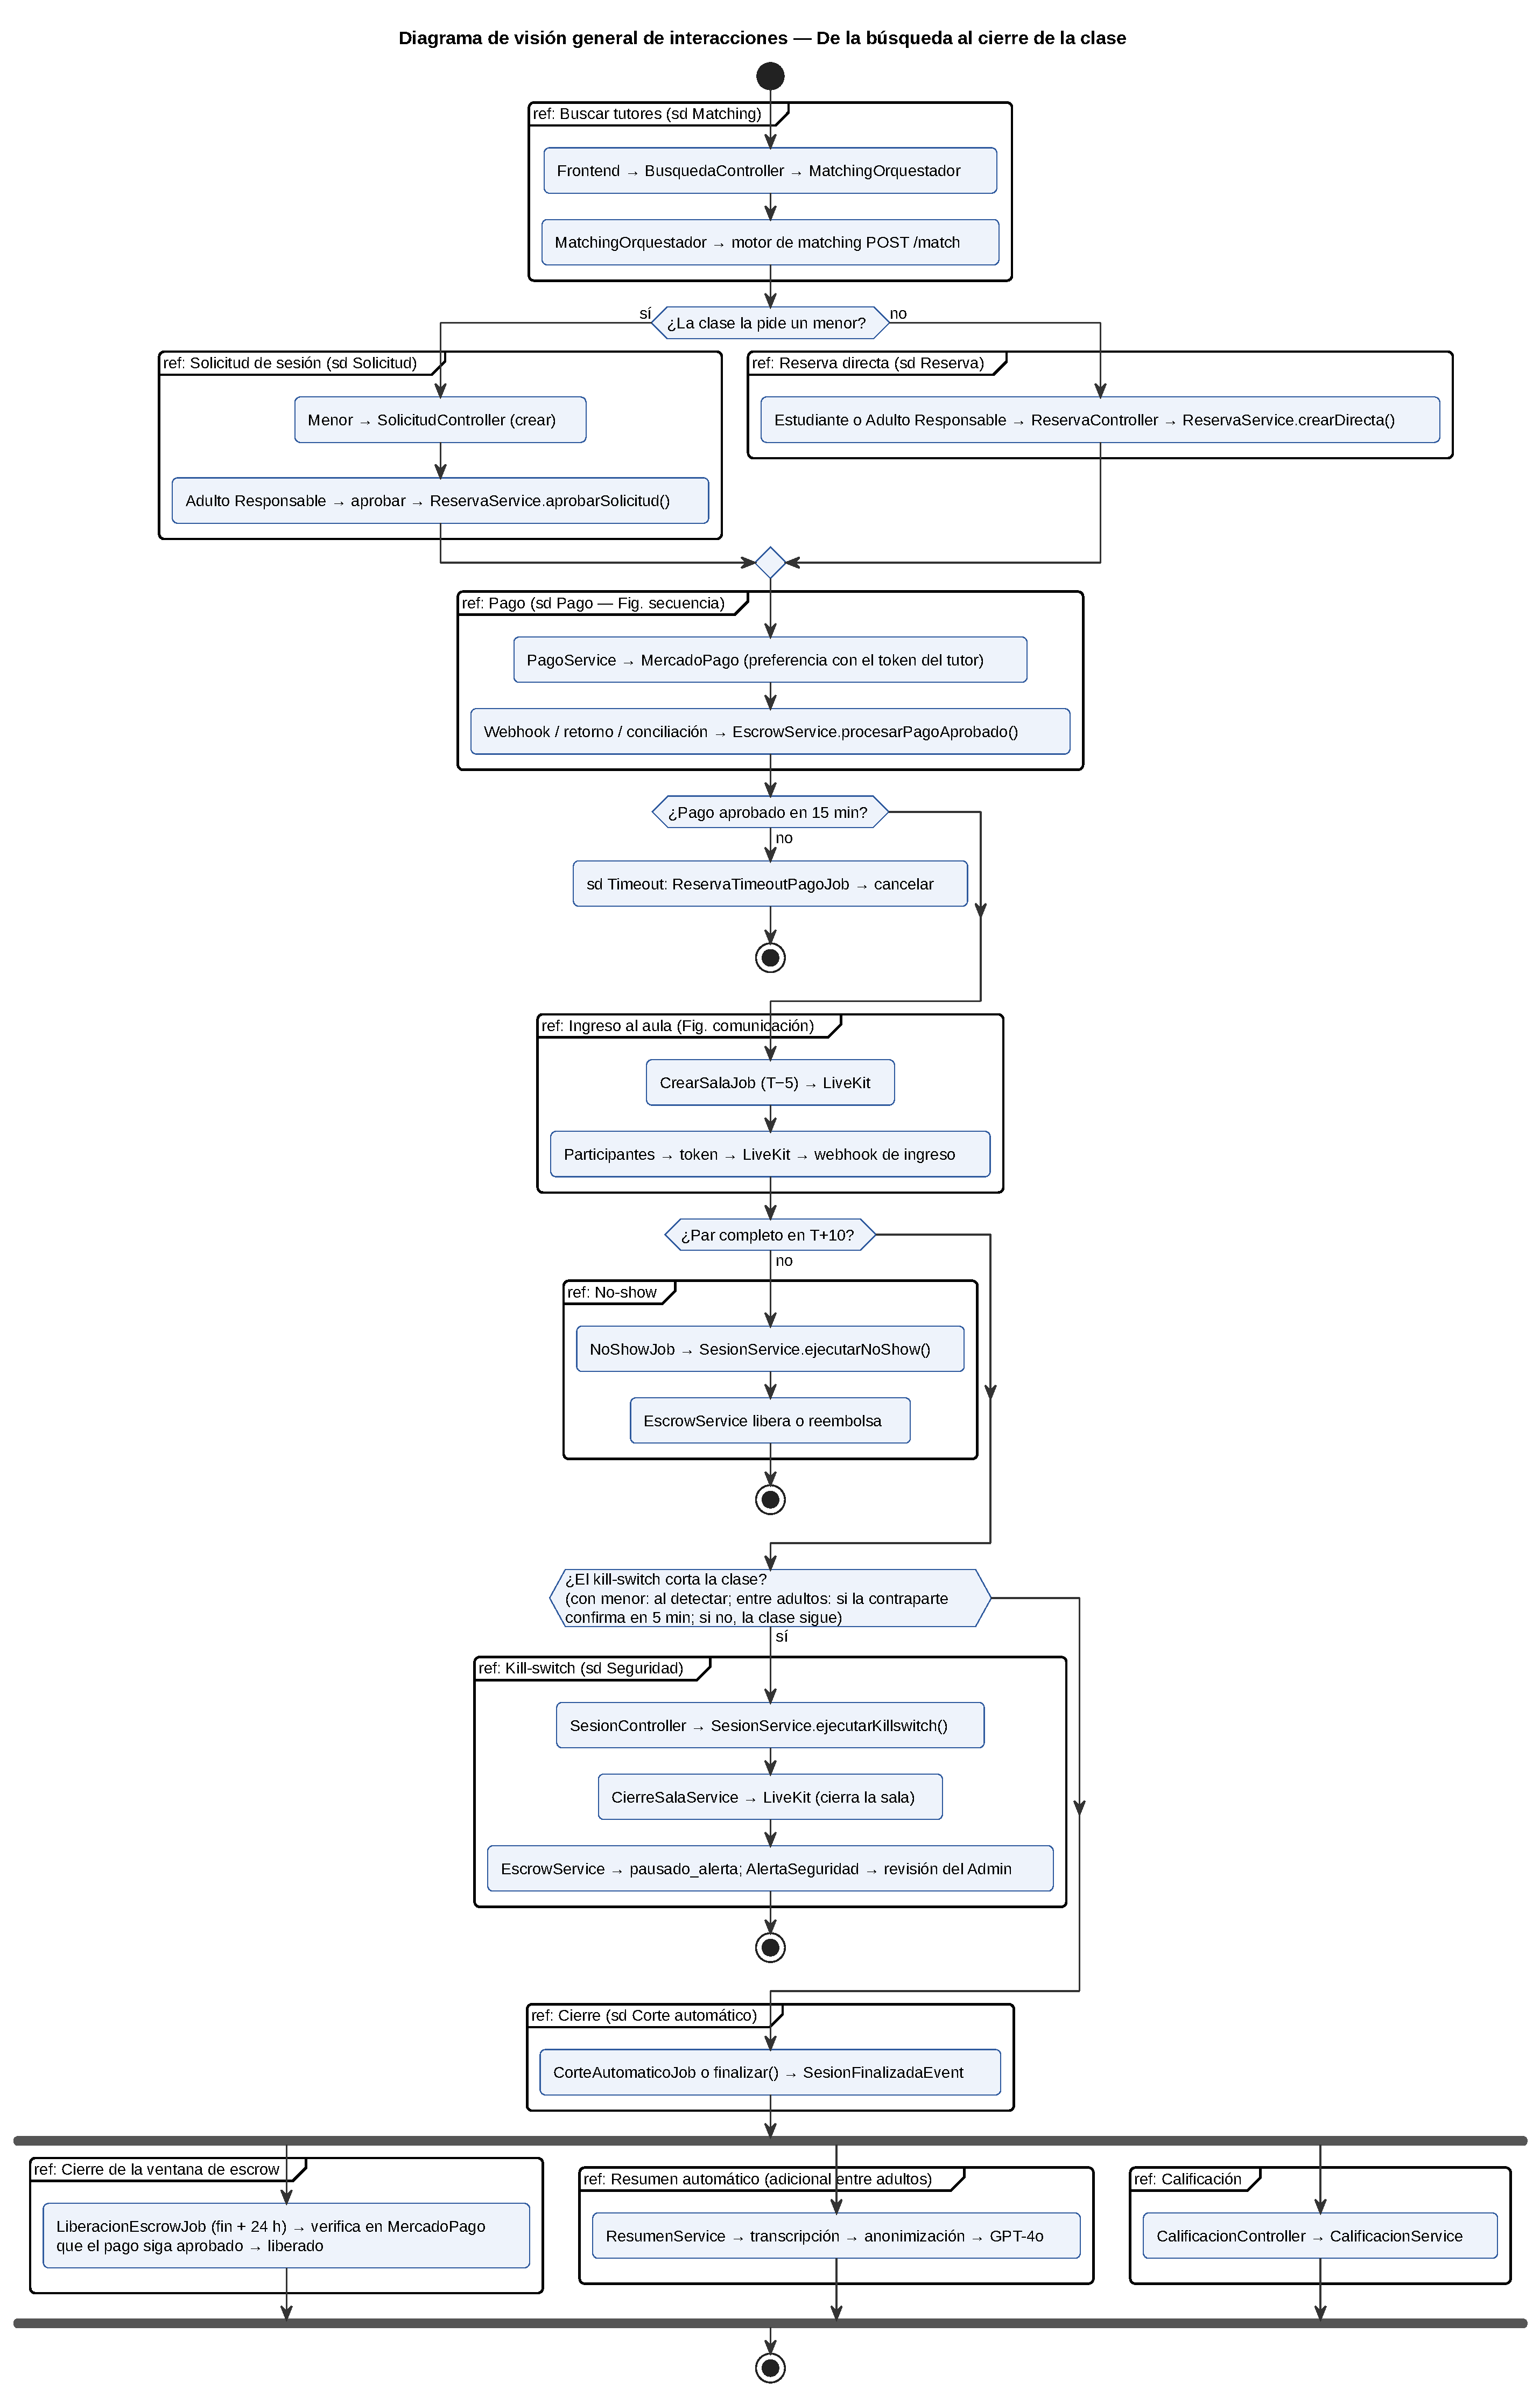
\includegraphics[width=\textwidth,height=0.8\textheight,keepaspectratio]{figuras/uml/07-vision-interacciones}
    \caption{Diagrama de visión general de interacciones}
    \label{fig:uml-vision-general}
\end{figure}

\section{Diagrama de clases}

La figura~\ref{fig:uml-clases} presenta las entidades del dominio
agrupadas por módulo, con sus atributos principales, sus enumeraciones de
estado y sus multiplicidades; es la vista detallada del modelo que resume
la sección~\ref{sec:modelo-datos}. \texttt{Usuario} concentra las
identidades: una Reserva lo referencia tres veces (pagador, beneficiario y
tutor), un menor se vincula con su Adulto Responsable por una
autorreferencia y \texttt{Admin} es una entidad aparte, vinculada a un
usuario, con uno de dos roles. Un \texttt{Paquete} agrupa cuatro Reservas,
y la cuenta de MercadoPago conectada del tutor (\texttt{CuentaMpTutor})
guarda su token cifrado.

\begin{figure}[H]
    \centering
    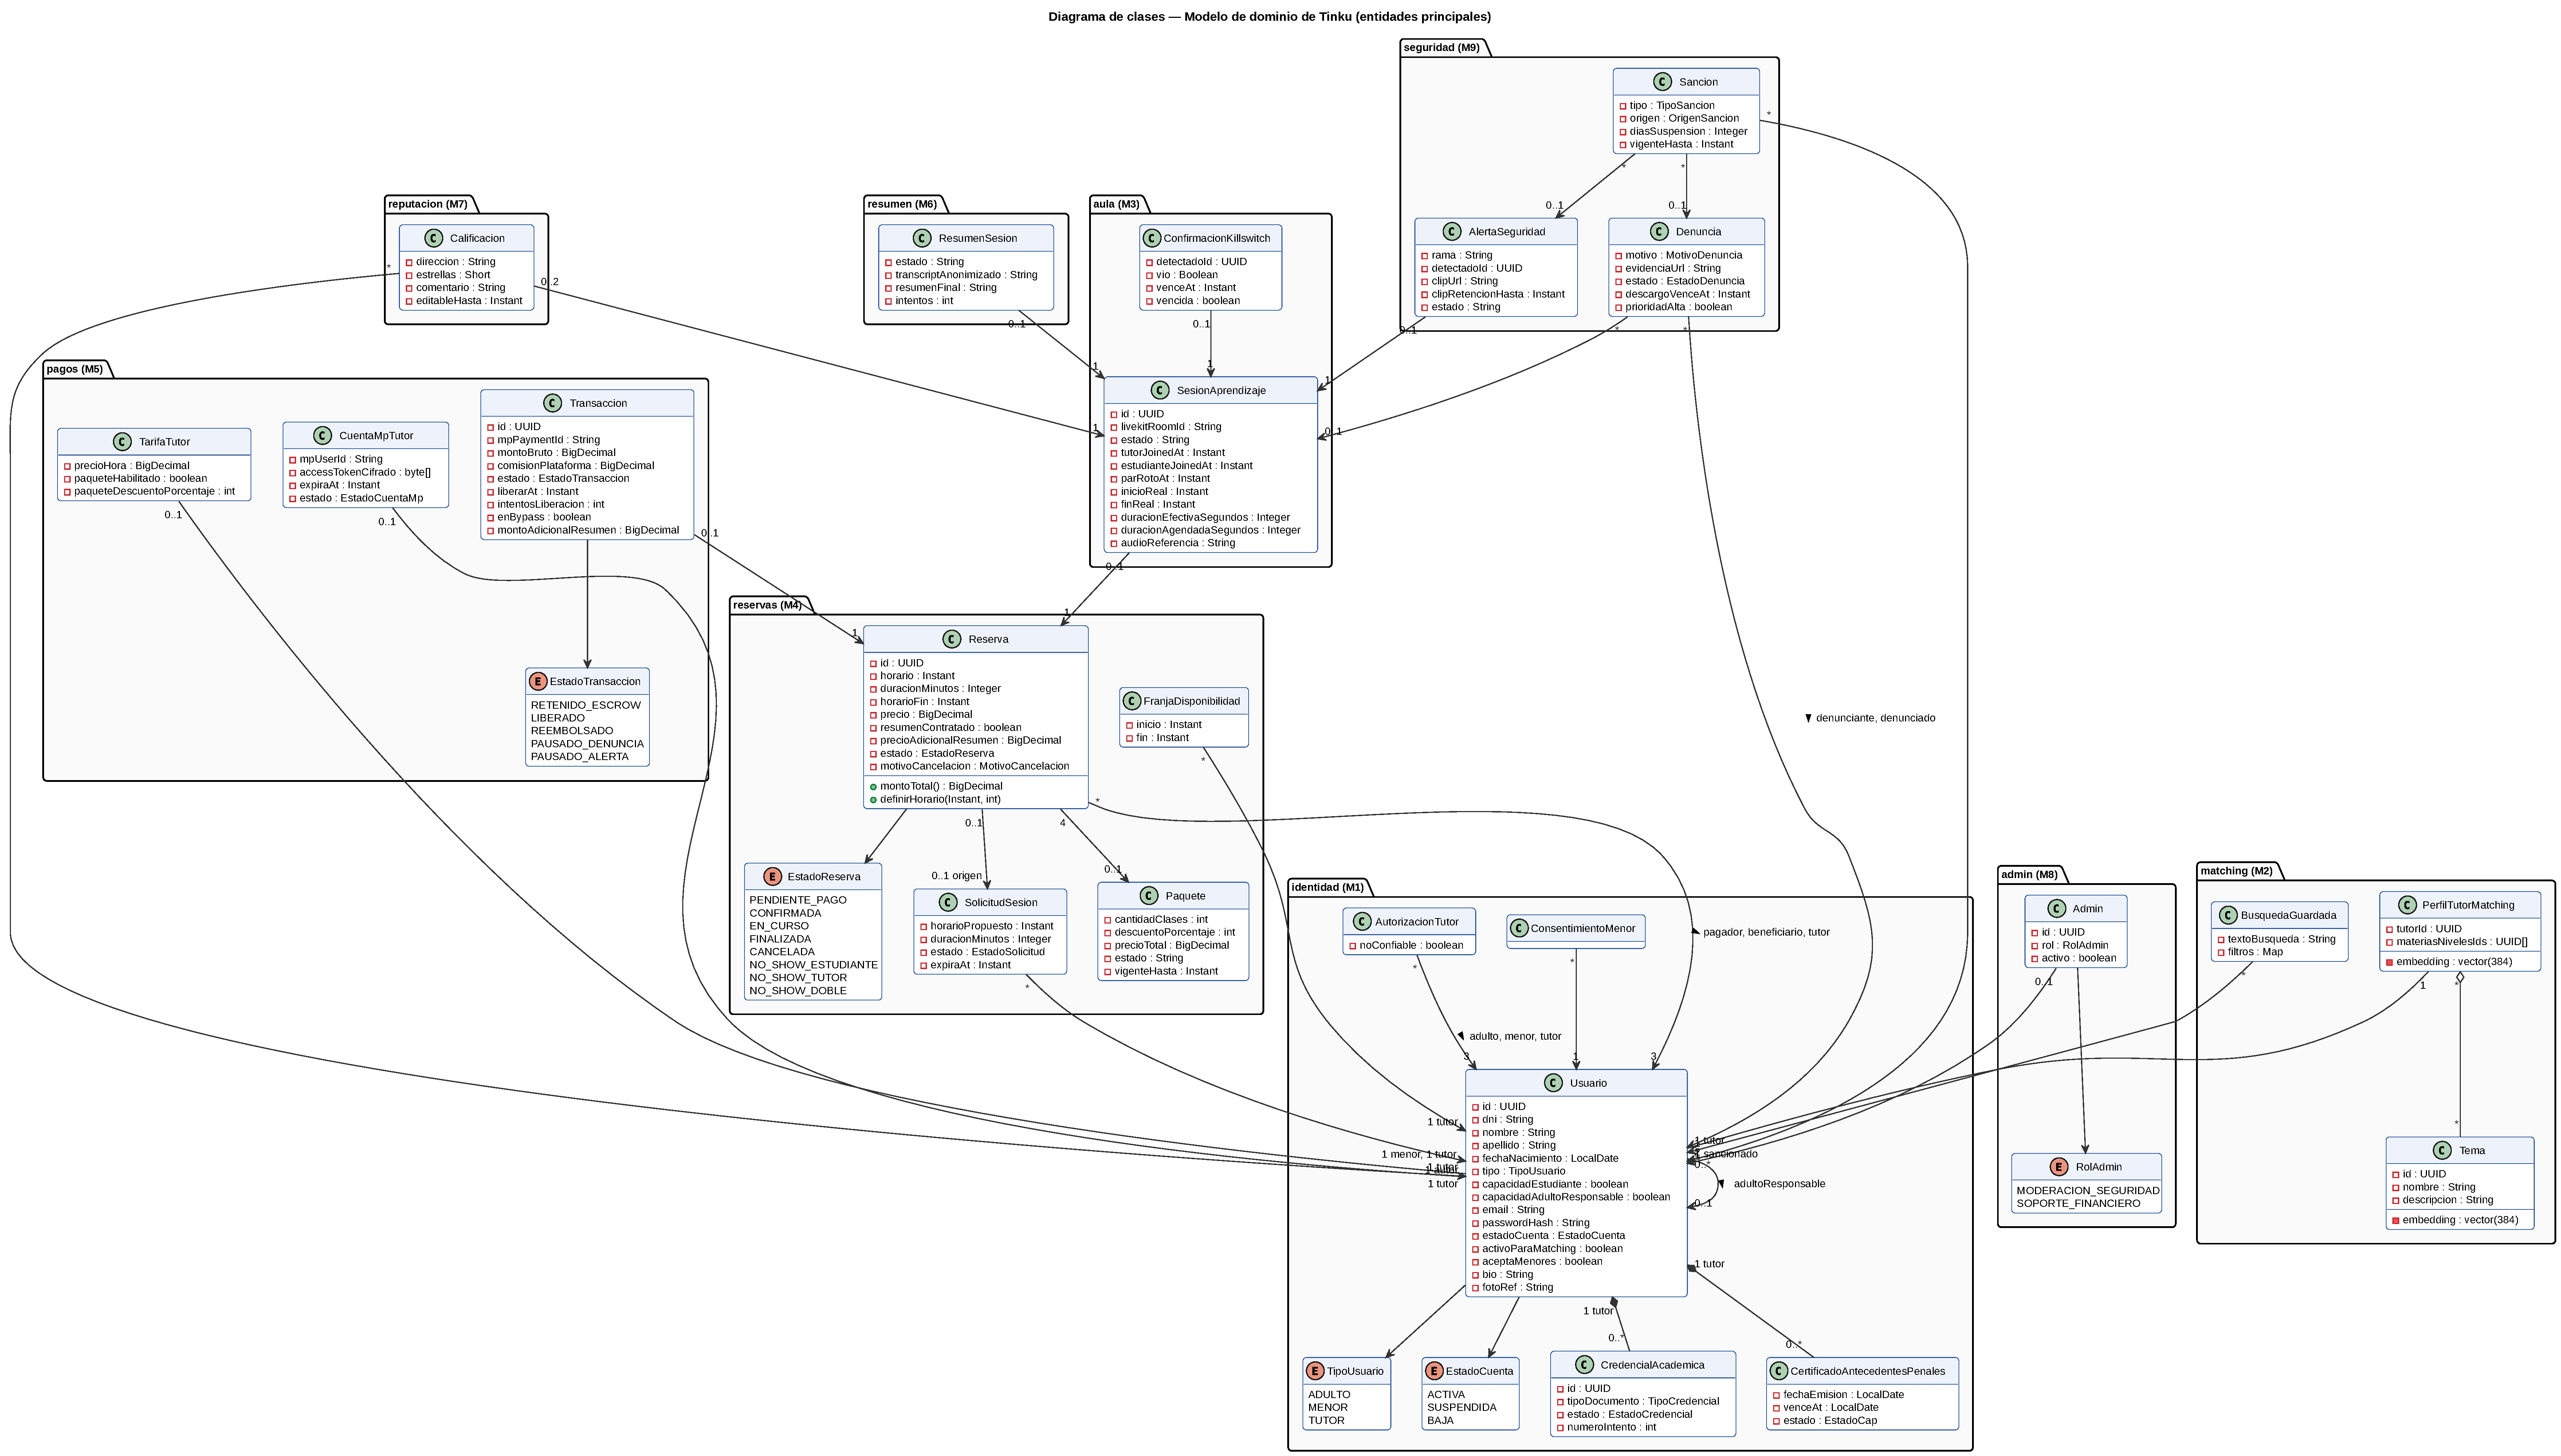
\includegraphics[width=\textwidth,height=0.8\textheight,keepaspectratio]{figuras/uml/08-clases}
    \caption{Diagrama de clases del modelo de dominio}
    \label{fig:uml-clases}
\end{figure}

\section{Diagrama de componentes}

La figura~\ref{fig:uml-componentes} detalla la vista de la
figura~\ref{fig:arquitectura}: el monolito modular Spring Boot con sus
nueve módulos y el planificador Quartz, el frontend Next.js con el
clasificador del kill-switch, el motor de \gls{matching} en Python (el
único proceso propio separado), PostgreSQL con pgvector, el respaldo
cifrado hacia Cloudflare R2 y los servicios externos. Las flechas
punteadas entre módulos son eventos de dominio en memoria; el único
ingreso desde internet es el túnel de Cloudflare.

\begin{figure}[H]
    \centering
    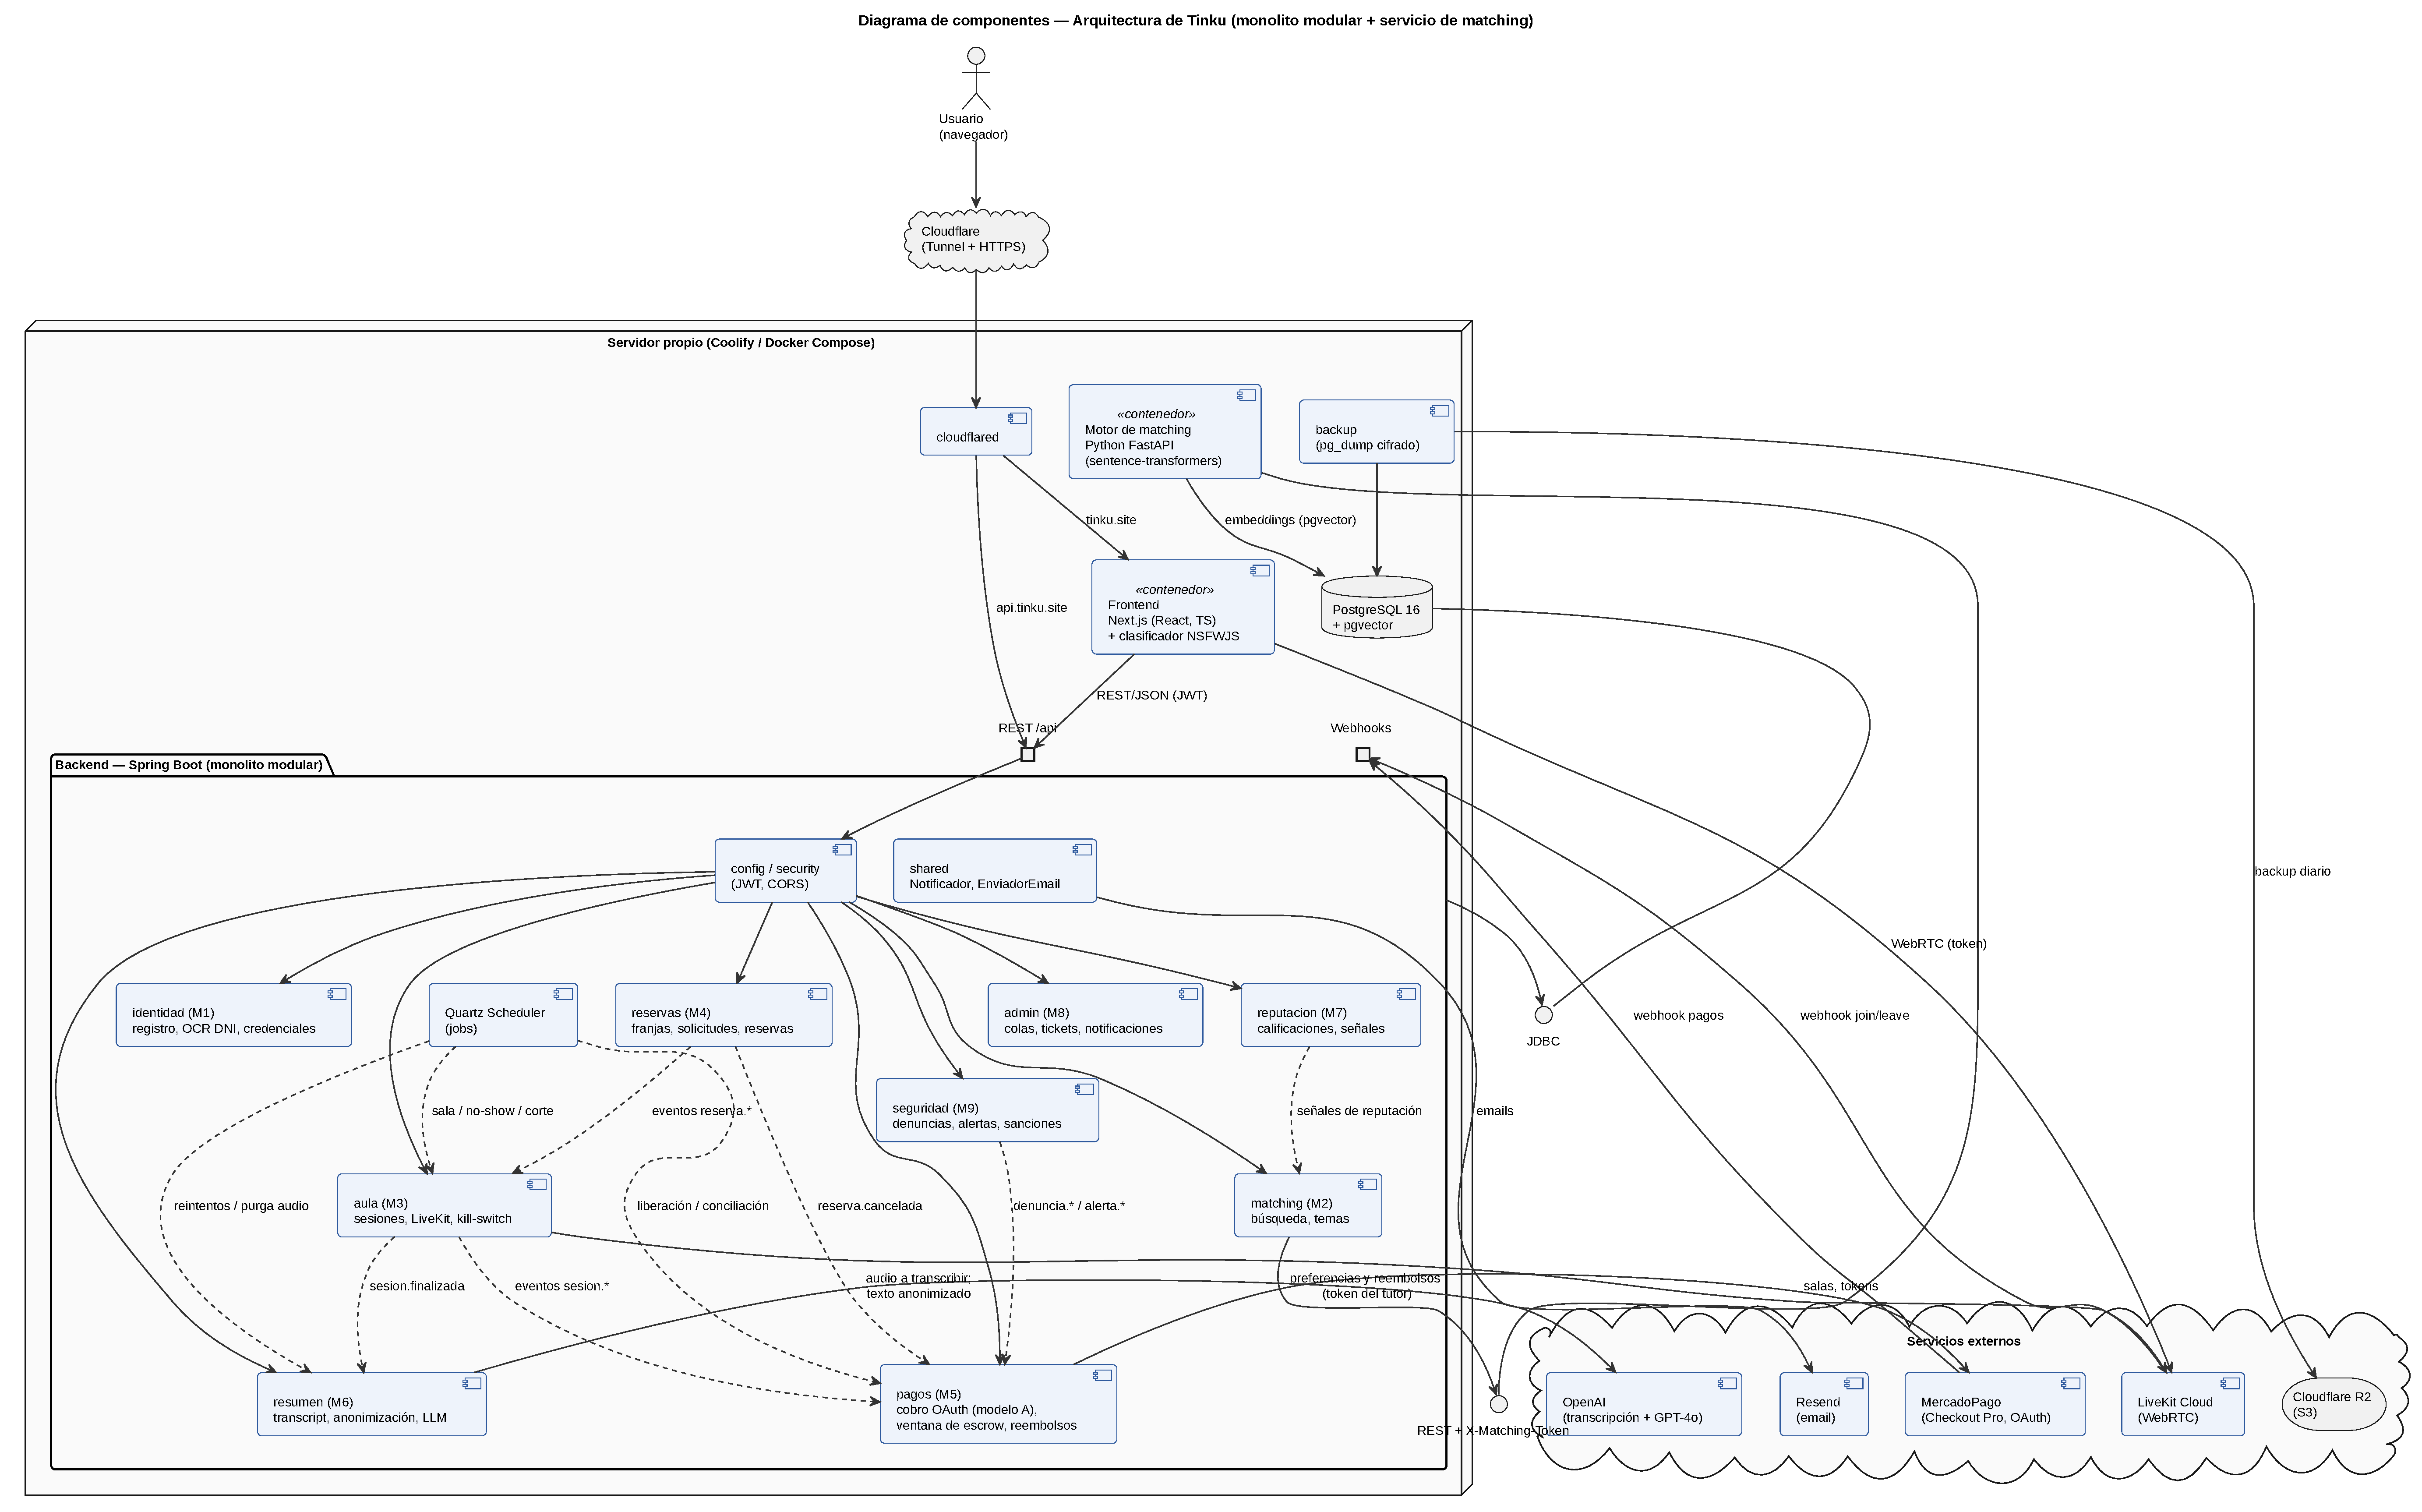
\includegraphics[width=\textwidth,height=0.8\textheight,keepaspectratio]{figuras/uml/09-componentes}
    \caption{Diagrama de componentes de \sistema{}}
    \label{fig:uml-componentes}
\end{figure}
